\chapter{Random Variable}

\section{The Definition of a Random Variable}

\begin{definition}[Random Variable]\index{random variable}
  A \emph{random variable} (r.v.) is a function \(X: \Omega \to \mathbb{R}\) that assigns a real number to each outcome in the sample space \(\Omega\).
\end{definition}

\begin{remark}
  Let \((\Omega, \mathcal{F}, P)\) be a probability space. In measure-theoretic probability, a random variable is defined as a measurable function \(X: \Omega \to \mathbb{R}\), s.t. \(X^{-1}(B) = \{\omega \in \Omega : X(\omega) \in B\} \in \mathcal{F}\) for all \(B \in \mathcal{B}(\mathbb{R})\), where \(\mathcal{B}(\mathbb{R})\) is the Borel \(\sigma\)-algebra on \(\mathbb{R}\).
\end{remark}

\begin{definition}[Discrete Random Variable]\index{discrete random variable}
  A random variable \(X\) is said to be \emph{discrete} type if the number of values it can take is finite or countably infinite.
\end{definition}

\section{Discrete Random Variables}

\begin{definition}[Probability Mass Function]\index{probability mass function}
  For a discrete random variable \(X\), the \emph{probability (mass) function} (p.f.) is defined as
  \[
    p(x) = P(X = x), \quad x \in \mathbb{R}.
  \]
\end{definition}

\begin{proposition}
  The function \(p(x)\) satisfies the following properties:
  \begin{enumerate}
    \item \(p(x) \geq 0\) for all \(x \in \mathbb{R}\).
    \item \(\sum_{i = 1}^\infty p(x_i) = 1\), where \(\{x_i\}\) is the set of all possible values of \(X\).
  \end{enumerate}
\end{proposition}

\begin{example}
  Bob is shooting. Suppose that the probability of hitting the target is 0.1. Suppose that each shooting is independent. Let \(X\) be the number of hits in 5 shootings. What is the probability of the event that Bob hits the target at least four times, i.e., \(P\{X \geq 4\}\)?
\end{example}
\begin{solution}
  By Bernoulli trial, we have
  \[
    P\{X = k\} = \binom{5}{k} (0.1)^k (0.9)^{5-k}, \quad k = 0, 1, 2, 3, 4, 5.
  \]
  Therefore,
  \[
    P\{X \geq 4\} = P\{X = 4\} + P\{X = 5\} = 0.00045 + 0.00001 = 0.00046. \qedhere
  \]
\end{solution}

\begin{definition}[Bernoulli Distribution]\index{Bernoulli distribution}\index{two-point distribution}
  A discrete random variable \(X\) is said to have a \emph{Bernoulli distribution} (or \emph{two-point distribution}) with parameter \(p\) if its probability mass function is given by
  \[
    p(x) = \begin{cases}
      p, & x = 1, \\
      1 - p, & x = 0. \\
    \end{cases}
  \]
\end{definition}

\begin{definition}[Binomial Distribution]\index{binomial distribution}
  A discrete random variable \(X\) is said to have a \emph{binomial distribution} with parameters \(n\) and \(p (0 < p < 1)\) if its probability mass function is given by
  \[
    P(X = k) = \binom{n}{k} p^k (1 - p)^{n - k}, \quad k = 0, 1, 2, \dots, n.
  \]
  We denote this distribution by \(X \sim \mathrm{B}(n, p)\).
\end{definition}

\begin{proposition}
  Let \(X \sim \mathrm{B}(n, p)\). The probability mass function \(f(k) = P(X = k)\) is unimodal. The set of modes, denoted by \(\mathcal{K}^* = \arg\max_{k \in \{0, \dots, n\}} P(X = k)\), is determined as follows:
  \begin{enumerate}
    \item If \((n+1)p\) is not an integer, there is a unique mode \(k^* = \lfloor (n+1)p \rfloor\). The sequence \(P(X=k)\) strictly increases for \(k \le k^*\) and strictly decreases for \(k \ge k^*\).
    \item If \((n+1)p\) is an integer, there are two adjacent modes \(k_1^* = (n+1)p - 1\) and \(k_2^* = (n+1)p\). In this case, \(P(X=k)\) strictly increases for \(k \le k_1^*\), satisfies \(P(X=k_1^*) = P(X=k_2^*)\), and strictly decreases for \(k \ge k_2^*\).
  \end{enumerate}
\end{proposition}
\begin{proof}
  For \(k = 0, 1, \dots, n-1\), we have
  \[
    \frac{P(X = k + 1)}{P(X = k)} = \frac{\binom{n}{k + 1} p^{k + 1} (1 - p)^{n - k - 1}}{\binom{n}{k} p^k (1 - p)^{n - k}} = \frac{n - k}{k + 1} \cdot \frac{p}{1 - p}.
  \]
  Therefore, \(P(X = k + 1) > P(X = k)\) if and only if \(k < (n + 1)p - 1\), and \(P(X = k + 1) < P(X = k)\) if and only if \(k > (n + 1)p - 1\). The rest of the proof follows immediately. \qedhere
\end{proof}

\begin{theorem}[Poisson Limit Theorem]\index{Poisson limit theorem}
  Suppose that \(\lambda > 0\) is a constant and \(n\) is a positive integer. If \(\lim_{n \to \infty} np_n = \lambda\), then for any fixed \(k = 0, 1, 2, \dots\), we have
  \[
    \lim_{n \to \infty} \binom{n}{k} p^k (1 - p)^{n - k} = \frac{\lambda^k e^{-\lambda}}{k!}.
  \]
\end{theorem}

\begin{definition}[Poisson Distribution]\index{Poisson distribution}
  A discrete random variable \(X\) is said to have a \emph{Poisson distribution} with parameter \(\lambda > 0\) if its probability mass function is given by
  \[
    P(X = k) = \frac{\lambda^k e^{-\lambda}}{k!}, \quad k = 0, 1, 2, \dots.
  \]
  We denote this distribution by \(X \sim \mathrm{Poi}(\lambda)\).
\end{definition}

The sum of the probabilities of a Poisson distribution is
\[
  \sum_{k = 0}^\infty \frac{\lambda^k e^{-\lambda}}{k!} = e^{-\lambda} \sum_{k = 0}^\infty \frac{\lambda^k}{k!} = e^{-\lambda} e^{\lambda} = 1.
\]

\begin{definition}[Geometric Distribution]\index{geometric distribution}
  A discrete random variable \(X\) is said to have a \emph{geometric distribution} with parameter \(p\) if its probability mass function is given by
  \[
    P(X = k) = p (1 - p)^{k - 1}, \quad k = 1, 2, \dots.
  \]
  We denote this distribution by \(X \sim \mathrm{G}(p)\) (or \(X \sim \mathrm{Geom}(p)\)).  
\end{definition}

\begin{proposition}
  \(X \sim \mathrm{G}(p)\) if and only if \(P\{X > m + n | X > m\} = P\{X > n\}\) for any \(m, n = 0, 1, 2, \dots\). This property is called the \emph{memoryless property} of the geometric distribution.
\end{proposition}

\begin{proof}
  \((\Rightarrow)\) Suppose that \(X \sim \mathrm{G}(p)\). For any \(m, n = 0, 1, 2, \dots\), we have
  \[
    P\{X > m + n | X > m\} = \frac{P\{X > m + n\}}{P\{X > m\}} = \frac{(1 - p)^{m + n}}{(1 - p)^m} = (1 - p)^n.
  \]
  Since
  \[
    P\{X > n\} = \sum_{k = n + 1}^\infty p (1 - p)^{k - 1} = p \cdot \frac{(1 - p)^n}{1 - (1 - p)} = (1 - p)^n,
  \]
  we have \(P\{X > m + n | X > m\} = P\{X > n\}\).

  \((\Leftarrow)\) Suppose that \(P\{X > m + n | X > m\} = P\{X > n\}\) for any \(m, n = 0, 1, 2, \dots\). Let \(g(n) = P(X > n)\). Then we have
  \[
    g(m + n) = P\{X > m + n | X > m\} P(X > m) = g(n) g(m).
  \]
  By mathematical induction, we can show that \(g(n) = g(1)^n\) for any \(n = 0, 1, 2, \dots\). Because \(X\) is a discrete random variable, we have \(0 \leq g(1) \leq 1\). Let \(p = 1 - g(1) \in (0, 1)\), then \(P(X > n) = (1 - p)^n\) for any \(n = 0, 1, 2, \dots\). It follows that \(P(X = k) = P(X > k - 1) - P(X > k) = p (1 - p)^{k - 1}\) for \(k = 1, 2, \dots.\)
\end{proof}

\begin{definition}[Pascal Distribution]\index{Pascal distribution}
  A discrete random variable \(X\) is said to have a \(k\)-th order \emph{Pascal distribution} (or \emph{Negative Binomial distribution}) if its probability mass function is given by
  \[
    P(X = n) = \binom{n - 1}{k - 1} p^k (1 - p)^{n - k}, \quad n = k, k + 1, \dots.
  \]
\end{definition}

\begin{definition}[Hypergeometric Distribution]\index{hypergeometric distribution}
  A discrete random variable \(X\) is said to have a \emph{hypergeometric distribution} with parameters \(N\), \(M\), and \(n\) if its probability mass function is given by
  \[
    P\{X = m \vert N, M, n\} = \frac{\binom{M}{m} \binom{N - M}{n - m}}{\binom{N}{n}}, \quad m = 0, 1, \dots, \min\{M, n\},
  \]
  where \(N\) is the total number of items, \(M\) is the number of items with a certain property, and \(n\) is the number of items drawn without replacement.
\end{definition}

\section{Distribution Function}

\begin{definition}[Distribution Function]\index{distribution function}\index{cumulative distribution function}
  The function \(F(x) = P(X \leq x) (-\infty < x < \infty)\) is called the \emph{(cumulative) distribution function} (c.d.f.\@ or d.f.) of the random variable \(X\), denoted by \(X \sim F(x)\) or \(F_X(X)\).
\end{definition}

\begin{proposition}
  The d.f.\@ \(F(x)\) satisfies the following properties:
  \begin{enumerate}
    \item \(F(x)\) is non-decreasing, i.e., \(F(x_1) \leq F(x_2)\) for any \(x_1 < x_2\).
    \item \(\lim_{x \to -\infty} F(x) = 0\) and \(\lim_{x \to \infty} F(x) = 1\).
    \item \(F(x)\) is right-continuous, i.e., \(\lim_{h \to 0^+} F(x + h) = F(x)\) for any \(x\).
  \end{enumerate}
\end{proposition}

We can calculate the following probabilities by using the d.f.\@ \(F(x)\):
\begin{align*}
  P(x_1 < X \leq x_2) & = P(X \leq x_2) - P(X \leq x_1) = F(x_2) - F(x_1), \\
  P(X < x) & = P(X \leq x) - P(X = x) \\
  & = F(x) - [F(x) - \lim_{h \to 0^+} F(x - h)] = \lim_{h \to 0^+} F(x - h) = F(x^-), \\
  P(X > x) & = 1 - P(X \leq x) = 1 - F(x).
\end{align*}

\begin{example}
  Suppose that the d.f.\@ of a r.v.\@ \(X\) is given by
  \[
    F(x) = \begin{cases}
      0, & x < -1, \\
      a, & -1 \leq x < 1, \\
      \frac{2}{3} - a, & 1 \leq x < 2, \\
      a + b, & x \geq 2,
    \end{cases}
  \]
  and \(F(1) = \frac{1}{2}\). Find the values of \(a\) and \(b\).
\end{example}
\begin{solution}
  Since \(F(1) = \frac{2}{3} - a = \frac{1}{2}\), we have \(a = \frac{1}{6}\). Since \(\lim_{x \to \infty} F(x) = a + b = 1\), we have \(b = \frac{5}{6}\).
\end{solution}

The relationship between the p.f.\@ \(p(x)\) and the d.f.\@ \(F(x)\) of a discrete r.v.\@ is
\[
  p(x) = P(X = x) = F(x) - \lim_{h \to 0^+} F(x - h) = F(x) - F(x^-).
\]

\section{Continuous Random Variables}

\begin{definition}[Continuous Random Variable]\index{continuous random variable}\index{probability density function}
  A random variable \(X\) is said to be \emph{continuous random variable} if there is a non-negative function \(f(x)\) defined on \(\mathbb{R}\) such that
  \[
    F(x) = P(X \leq x) = \int_{-\infty}^x f(t)\,\mathrm{d}t, \quad -\infty < x < \infty.
  \]
  \(f(x)\) is called the \emph{probability density function} (p.d.f.) of \(X\).
\end{definition}

\(X\) is called a \emph{continuous} r.v.\@ because \(F(x)\) is continuous. We can show that \(P(X = x) = 0\) for any \(x \in \mathbb{R}\) if \(X\) is a continuous r.v.
\begin{proof}
  For any \(x \in \mathbb{R}\), the event \(\{X = x\}\) can be expressed as a limit of nested intervals:
  \[
    \{X = x\} = \{x \leq X \leq x\} = \bigcap_{n=1}^{\infty} \left\{x - \frac{1}{n} < X \leq x\right\}.
  \]
  Note that \(A_n \downarrow A\), i.e., $A_1 \supseteq A_2 \supseteq \cdots$ where $A_n = \{x - \frac{1}{n} < X \leq x\}$, and their intersection is exactly $\{X = x\}$. By continuity of probability from above:
  \[
    P(X = x) = \lim_{n \to \infty} P\!\left(x - \frac{1}{n} < X \leq x\right).
  \]
  Now, using the c.d.f.\@ definition directly, the probability of any half-open interval is:
  \begin{align*}
    P\!\left(x - \frac{1}{n} < X \leq x\right) & = F(x) - F\!\left(x - \frac{1}{n}\right) \\
    & = \int_{-\infty}^{x} f(t)\,\mathrm{d}t - \int_{-\infty}^{x - 1/n} f(t)\,\mathrm{d}t = \int_{x - 1/n}^{x} f(t)\,\mathrm{d}t.
  \end{align*}
  Since $f$ is non-negative and integrable, and the interval \([x - \frac{1}{n},\, x]\) has length \(\frac{1}{n} \to 0\):
  \[
    0 \leq P(X = x) = \lim_{n\to\infty} \int_{x-1/n}^{x} f(t)\,\mathrm{d}t = \int_{x}^{x} f(t)\,\mathrm{d}t = 0.
  \]
  The last equality follows because the integral of any locally integrable function over a set of measure zero (a single point) is zero.
\end{proof}

We can calculate the following probabilities by using the p.d.f.\@ \(f(x)\):
\begin{align*}
  P(x_1 < X \leq x_2) & = F(x_2) - F(x_1) = \int_{x_1}^{x_2} f(t)\,\mathrm{d}t, \\
  P(X < x) & = P(X \leq x) - P(X = x) = F(x) - 0 = \int_{-\infty}^x f(t)\,\mathrm{d}t, \\
  P(X > x) & = 1 - P(X \leq x) = 1 - F(x) = \int_x^\infty f(t)\,\mathrm{d}t, \\
  P(X \in I) & = \int_I f(t)\,\mathrm{d}t, \quad \text{for any interval } I.
\end{align*}

The relationship between the p.d.f.\@ \(f(x)\) and the d.f.\@ \(F(x)\) of a continuous r.v.\@ is given by the Fundamental Theorem of Calculus:
\[
  F'(x) = f(x).
\]

\begin{example}
  Suppose that the p.d.f.\@ of r.v.\@ \(X\) is given by
  \[
    f(x) = \begin{cases}
      0, & x \leq 0, \\
      k e^{-3x}, & x > 0.
    \end{cases}
  \]
  \begin{enumerate}
    \item Determine the value of \(k\).
    \item Find the corresponding d.f.\@ \(F(x)\).
    \item Calculate \(P\{X > 0.1\}\).
  \end{enumerate}
\end{example}
\begin{solution}
  \begin{enumerate}
    \item Since \(\int_{-\infty}^\infty f(x)\,\mathrm{d}x = 1\), we have
    \[
      \int_{-\infty}^\infty f(x)\,\mathrm{d}x = \int_0^\infty k e^{-3x}\,\mathrm{d}x = \frac{k}{3} = 1 \implies k = 3.
    \]
    \item For \(x > 0\), we have
    \[
      F(x) = \int_{-\infty}^x f(t)\,\mathrm{d}t = \int_0^x 3 e^{-3t}\,\mathrm{d}t = 1 - e^{-3x}.
    \]
    For \(x \leq 0\), we have \(F(x) = P(X \leq x) =  0\). Therefore,
    \[
      F(x) = \begin{cases}
        0, & x \leq 0, \\
        1 - e^{-3x}, & x > 0.
      \end{cases}
    \]
    \item We have
    \[
      P\{X > 0.1\} = 1 - P\{X \leq 0.1\} = 1 - F(0.1) = 1 - (1 - e^{-0.3}) = e^{-0.3}. \qedhere
    \]
  \end{enumerate}
\end{solution}

\begin{example}
  Determine the constants \(A\) and \(B\) such that the function
  \[
    F(x) = \begin{cases}
      A e^{x}, & x < 0, \\
      B - A e^{-x}, & x \geq 0,
    \end{cases}
  \]
  is a d.f.\@ of a continuous r.v.\@ \(X\), and find the corresponding p.d.f.\@ \(f(x)\).
\end{example}

\begin{solution}
  Since \(F(x)\) is a d.f.\@, we have
  \[
    \lim_{x \to \infty} F(x) = \lim_{x \to \infty} (B - A e^{-x}) = B = 1.
  \]
  Since \(F(x)\) is continuous at \(x = 0\), we have
  \[
    \lim_{x \to 0^-} F(x) = \lim_{x \to 0^+} F(x) \implies A = B - A \implies A = \frac{1}{2}.
  \]
  Therefore,
  \[
    F(x) = \begin{cases}
      \frac{1}{2} e^{x}, & x < 0, \\
      1 - \frac{1}{2} e^{-x}, & x \geq 0,
    \end{cases}
  \]
  and
  \[
    f(x) = F'(x) = \begin{cases}
      \frac{1}{2} e^{x}, & x < 0, \\
      \frac{1}{2} e^{-x}, & x \geq 0.
    \end{cases} \qedhere
  \]
\end{solution}

\begin{remark}
  Note that for continuous r.v.\@ \(X\), the p.d.f.\@ \(f(x)\) is not the probability of the event \(\{X = x\}\). In fact, \(P(X = x) = 0\) for any \(x\), while
  \[
    f(x) = \lim_{h \to 0^+} \frac{F(x + h) - F(x)}{h} = \lim_{h \to 0^+} \frac{P(x < X \leq x + h)}{h}.
  \]
\end{remark}

\begin{definition}[Uniform Distribution]\index{uniform distribution}
  The distribution of a random variable \(X\) is called the \emph{uniform distribution} on the interval \((a, b)\) if its p.d.f.\@ is given by
  \[
    f(x) = \begin{cases}
      \frac{1}{b - a}, & a < x < b, \\
      0, & \text{otherwise}.
    \end{cases}
  \]
  We denote this distribution by \(X \sim \mathrm{U}(a, b)\).
\end{definition}

The d.f.\@ of \(X \sim \mathrm{U}(a, b)\) is given by
\[
  F(x) = \begin{cases}
    0, & x < a, \\
    \frac{x - a}{b - a}, & a \leq x < b, \\
    1, & x \geq b.
  \end{cases}
\]

\begin{example}
  Suppose taht \(X \sim \mathrm{U}(a, b)\), and \(P(0 < X < 3) = \frac{1}{4}\), \(P(X > 4) = \frac{1}{2}\). Find the p.d.f.\@ of \(X\) and the values of \(P(1 < X < 5)\).
\end{example}

\begin{solution}
  Since \(P(0 < X < 3) = \frac{1}{4}\), we have \(a < 3\); since \(P(X > 4) = \frac{1}{2}\), we have \(b > 4\), and
  \[
    P(X > 4) = \frac{b - 4}{b - a} = \frac{1}{2} \implies a + b = 8.
  \]
  \begin{enumerate}
    \item If \(a \geq 0\), we have
    \[
      P(0 < X < 3) = \frac{3 - a}{b - a} = \frac{1}{4} \implies 3a + b = 12.
    \]
    Solving the equations, we have \(a = 2\) and \(b = 6\). The p.d.f.\@ of \(X\) is given by
    \[
      f(x) = \begin{cases}
        \frac{1}{4}, & 2 < x < 6, \\
        0, & \text{otherwise}.
      \end{cases}
    \]
    Therefore,
    \[
      P(1 < X < 5) = \int_1^5 f(x)\,\mathrm{d}x = \int_2^5 \frac{1}{4}\,\mathrm{d}x = \frac{3}{4}.
    \]
    \item If \(a < 0\), we have
    \[
      P(0 < X < 3) = \frac{3}{b - a} = \frac{1}{4} \implies b - a = 12.
    \]
    Solving the equations, we have \(a = -2\) and \(b = 10\). The p.d.f.\@ of \(X\) is given by
    \[
      f(x) = \begin{cases}
        \frac{1}{12}, & -2 < x < 10, \\
        0, & \text{otherwise}.
      \end{cases}
    \]
    Therefore,
    \[
      P(1 < X < 5) = \int_1^5 f(x)\,\mathrm{d}x = \int_1^5 \frac{1}{12}\,\mathrm{d}x = \frac{1}{3}. \qedhere
    \]
  \end{enumerate}
\end{solution}

\begin{definition}[Exponential Distribution]\index{exponential distribution}
  The distribution of a random variable \(X\) is called the \emph{exponential distribution} with parameter \(\lambda > 0\) if its p.d.f.\@ is given by
  \[
    f(x) = \begin{cases}
      \lambda e^{-\lambda x}, & x > 0, \\
      0, & x \leq 0.
    \end{cases}
  \]
  We denote this distribution by \(X \sim \mathrm{Exp}(\lambda)\).
\end{definition}

The d.f.\@ of \(X \sim \mathrm{Exp}(\lambda)\) is given by
\[
  F(x) = \begin{cases}
    1 - e^{-\lambda x}, & x > 0, \\
    0, & x \leq 0.
  \end{cases}
\]

\begin{proposition}
  \(X \sim \mathrm{Exp}(\lambda)\) if and only if \(P\{X \geq s + t | X  \geq s\} = P\{X \geq t\}\) for any \(s, t > 0\). This property is called the \emph{memoryless property} of the exponential distribution.
\end{proposition}

\begin{proof}
  \((\Rightarrow)\) Suppose that \(X \sim \mathrm{Exp}(\lambda)\). For any \(s, t > 0\), we have
  \[
    P\{X \geq s + t | X  \geq s\} = \frac{P\{X \geq s + t\}}{P\{X \geq s\}} = \frac{e^{-\lambda (s + t)}}{e^{-\lambda s}} = e^{-\lambda t}.
  \]
  Since
  \[
    P\{X \geq t\} = e^{-\lambda t},
  \]
  we have \(P\{X \geq s + t | X  \geq s\} = P\{X \geq t\}\).

  \((\Leftarrow)\) Suppose that \(P\{X \geq s + t | X  \geq s\} = P\{X \geq t\}\) for any \(s, t > 0\). Let \(g(t) = P(X \geq t)\), which the survival function of \(X\). Then we have
  \[
    g(s + t) = P\{X \geq s + t | X  \geq s\} P(X \geq s) = g(t) g(s) \quad \text{for any } s, t > 0.
  \]
  This is a well-known functional equation (the multiplicative version of Cauchy's functional equation). 

  First, we rule out the trivial case where \(g(x) = 0\) everywhere. If \(g(t) = 0\) for some \(t > 0\), then \(g(t) = g(t/2 + t/2) = [g(t/2)]^2 = 0\). By continually halving \(t\), we would find \(g(x)=0\) for all \(x>0\). This represents a degenerate distribution (\(X=0\) almost surely), which is not a valid strictly positive continuous random variable. Thus, \(g(x) > 0\) for all \(x > 0\).

  Since \(g(x) > 0\), we can take the natural logarithm of both sides. Let \(h(x) = \ln(g(x))\):
  \[
    \ln(g(s+t)) = \ln(g(s)g(t)) \implies h(s+t) = h(s) + h(t).
  \]
  This is Cauchy's Additive Functional Equation. Because \(X\) is a continuous random variable, its c.d.f.\@ (and thus its survival function \(g(x)\)) is right-continuous and non-increasing. Consequently, \(h(x)\) is also non-increasing.

  It is a proven mathematical theorem that the only monotonic solutions to Cauchy's functional equation \(h(s+t) = h(s) + h(t)\) are linear functions of the form:
  \[
    h(x) = cx
  \]
  for some constant \(c\).

  Substituting \(h(x)\) back in terms of \(g(x)\):
  \[
    \ln(g(x)) = cx \implies g(x) = e^{cx}.
  \]

  Because \(g(x)\) is a survival probability, it cannot exceed \(1\) and must decrease to \(0\) as \(x \to \infty\). Since \(g(x) \leq 1\), \(c\) must be \(\leq 0\). Since \(\lim_{x \to \infty} g(x) = 0\) (a requirement for a proper random variable), \(c\) cannot be \(0\).

  Therefore, \(c\) must be strictly negative. Let us define \(c = -\lambda\) where \(\lambda > 0\). We then have:
  \[
    g(x) = P(X \geq x) = e^{-\lambda x}.
  \]
  This is exactly the survival function of an Exponential distribution with rate parameter $\lambda$. Hence, $X \sim \mathrm{Exp}(\lambda)$.
\end{proof}

\begin{example}
  The lifetime (in years) of a radio has an exponential distribution with parameter \(\lambda = 0.1\). If we buy a five-year-old radio, what is the probability that it will work for less than 10 additional years?
\end{example}

\begin{solution}
  Let \(X\) be the total lifetime of the radio, then \(X \sim \mathrm{Exp}(0.1)\). We seek
  \begin{align*}
    P(X \leq 15 | X > 5) & = 1 - P(X > 15 | X > 5) = 1 - P(X > 10) \\
    & = P(X \leq 10) = 1 - e^{-0.1 \cdot 10} = 1 - e^{-1}. \qedhere
  \end{align*}
\end{solution}

\paragraph{Relationship between Poisson and Exponential Distributions.} Suppose the number of the occurrences of a certain event \(N(t)\) in a time interval of length \(t\) follows a Poisson distribution with parameter \(\lambda t\), i.e., \(N(t) \sim \mathrm{Poi}(\lambda t)\). Then the waiting time \(T\) until the first occurrence of the event has an exponential distribution with parameter \(\lambda\), i.e., \(T \sim \mathrm{Exp}(\lambda)\). In fact, we have
\[
  P(T > t) = P\{N(t) = 0\} = \frac{(\lambda t)^0}{0!} e^{-\lambda t} = e^{-\lambda t},
\]
thus \(P(T \leq t) = 1 - e^{-\lambda t}\) for any \(t > 0\), which means \(T \sim \mathrm{Exp}(\lambda)\).

\begin{definition}[Normal Distribution]\index{normal distribution}\index{Gaussian distribution}
  The distribution of a random variable \(X\) is called the \emph{normal distribution} (or \emph{Gaussian distribution}) with parameters \(\mu\) and \(\sigma > 0\) if its p.d.f.\@ is given by
  \[
    f(x) = \frac{1}{\sqrt{2\pi} \sigma} e^{-\frac{(x - \mu)^2}{2\sigma^2}}, \quad -\infty < x < \infty.
  \]
  We denote this distribution by \(X \sim \mathrm{N}(\mu, \sigma^2)\). Particularly, if \(\mu = 0\) and \(\sigma = 1\), we call it the \emph{standard normal distribution}.
\end{definition}

The p.d.f.\@ of the standard normal distribution is given by
\[
  \phi(z) = \frac{1}{\sqrt{2\pi}} e^{-\frac{z^2}{2}}, \quad -\infty < z < \infty.
\]

\begin{figure}[tbp]
  \centering
    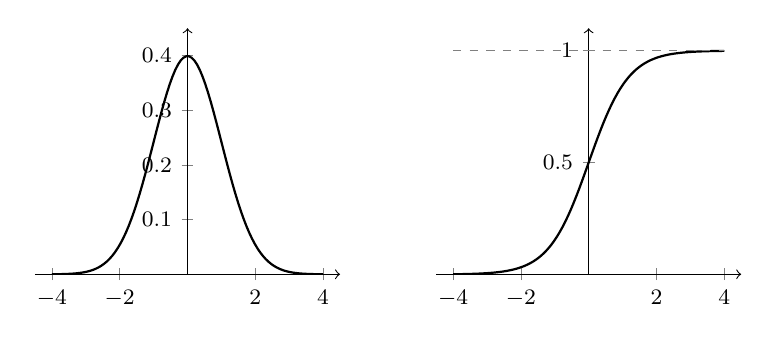
\begin{tikzpicture}[
      font=\footnotesize,
    ]
      \begin{axis}[
        name=pdf,
        width=0.45\linewidth,
        domain=-4:4,
        samples=100,
        axis lines=middle,
        inner axis line style={->},
        xmin=-4.5, xmax=4.5,
        ymax=0.45
      ]
        \addplot [thick, black] {exp(-0.5*x^2)/sqrt(2*pi)};
      \end{axis}
      
      \begin{axis}[
        at={(pdf.right of south east)},
        width=0.45\linewidth,
        xshift=0.1\linewidth,
        domain=-4:4,
        samples=100,
        axis lines=middle,
        inner axis line style={->},
        xmin=-4.5, xmax=4.5,
        ymax=1.1
      ]
        \addplot [thick, black] {1 / (1 + exp(-1.702 * x))};
        \draw[dashed, gray] (-4,1) -- (4,1);
      \end{axis}
    \end{tikzpicture}
  \caption{The p.d.f.\@ and d.f.\@ of the standard normal distribution.}
\end{figure}

The p.d.f.\@ of the normal distribution is obviously non-negative. We can show that the integral of the normal p.d.f.\@ is 1 by using the substitution \(z = \frac{x - \mu}{\sigma}\):
\[
  \int_{-\infty}^\infty \frac{1}{\sqrt{2\pi} \sigma} e^{-\frac{(x - \mu)^2}{2\sigma^2}}\,\mathrm{d}x = \frac{1}{\sqrt{2\pi}} \int_{-\infty}^\infty e^{-\frac{z^2}{2}}\,\mathrm{d}z \quad (z = \frac{x - \mu}{\sigma})
\]
By Theorem~\ref{thm:important_integrals}, we have
\[
  \int_{-\infty}^\infty e^{-\frac{z^2}{2}}\,\mathrm{d}z = 2 \int_{0}^{\infty} e^{-\frac{z^2}{2}}\,\mathrm{d}z = \sqrt{2\pi}.
\]
Therefore, the integral of the normal p.d.f.\@ is 1.

The d.f.\@ of \(X \sim \mathrm{N}(\mu, \sigma^2)\) is given by
\[
  F(x) = \frac{1}{\sqrt{2\pi} \sigma} \int_{-\infty}^x e^{-\frac{(t - \mu)^2}{2\sigma^2}}\,\mathrm{d}t, \quad -\infty < x < \infty,
\]
and the d.f.\@ of the standard normal distribution is given by
\[
  \Phi(z) = \frac{1}{\sqrt{2\pi}} \int_{-\infty}^z e^{-\frac{t^2}{2}}\,\mathrm{d}t, \quad -\infty < z < \infty.
\]

\begin{theorem}
  If \(X \sim \mathrm{N}(\mu, \sigma^2)\), then \(Z = \frac{X - \mu}{\sigma} \sim \mathrm{N}(0, 1)\).
\end{theorem}

\begin{proof}
  If \(X \sim \mathrm{N}(\mu, \sigma^2)\), and \(Z = \frac{X - \mu}{\sigma}\), then
  \begin{align*}
    P(Z \leq x) & = P\!\left(\frac{X - \mu}{\sigma} \leq x\right) \\
    & = P(X \leq \sigma x + \mu) \\
    & = \frac{1}{\sqrt{2\pi} \sigma} \int_{-\infty}^{\sigma x + \mu} e^{-\frac{(t - \mu)^2}{2\sigma^2}}\,\mathrm{d}t.
  \end{align*}
  Therefore,
  \[
    f_Z(x) = \frac{\mathrm{d}}{\mathrm{d}x} P(Z \leq x) = \frac{1}{\sqrt{2\pi}\sigma} e^{-\frac{(t - \mu)^2}{2\sigma^2}} \sigma \bigg|_{t = \sigma x + \mu} = \frac{1}{\sqrt{2\pi}} e^{-\frac{x^2}{2}}, \quad -\infty < x < \infty,
  \]
  which is the p.d.f.\@ of the standard normal distribution.
\end{proof}

\begin{example}
  Suppose that \(X \sim \mathrm{N}(10, 4)\). Find the value of \(P(10 < X < 13)\) and \(P(|X - 10| < 2)\).
\end{example}

\begin{solution}
  Since \(Z = \frac{X - 10}{2} \sim \mathrm{N}(0, 1)\), we have
  \[
    P(10 < X < 13) = P\!\left(0 < Z < \frac{3}{2}\right) = \Phi\!\left(\frac{3}{2}\right) - \Phi(0) = \Phi\!\left(\frac{3}{2}\right) - \frac{1}{2},
  \]
  and
  \[
    P(|X - 10| < 2) = P(8 < X < 12) = P\!\left(-1 < Z < 1\right) = \Phi(1) - \Phi(-1) = 2\Phi(1) - 1. \qedhere
  \]
\end{solution}

\begin{example}
  Suppose that \(X \sim \mathrm{N}(\mu, \sigma^2)\), \(P(X \leq -5) = 0.045\), and \(P(X \leq 3) = 0.618\). Find the values of \(\mu\) and \(\sigma\).
\end{example}

\begin{solution}
  Since \(P(X \leq -5) = 0.045\), we have
  \[
    P\!\left(\frac{X - \mu}{\sigma} \leq \frac{-5 - \mu}{\sigma}\right) = 0.045.
  \]
  Since \(P(X \leq 3) = 0.618\), we have
  \[
    P\!\left(\frac{X - \mu}{\sigma} \leq \frac{3 - \mu}{\sigma}\right) = 0.618.
  \]
  Let \(z_1 = \frac{-5 - \mu}{\sigma}\) and \(z_2 = \frac{3 - \mu}{\sigma}\). Then we have
  \[
    z_1 \approx -1.695, \quad z_2 \approx 0.300.
  \]
  Solving the equations, we have \(\mu = 1.80\) and \(\sigma \approx 4.01\).
\end{solution}

\section{Functions of Random Variables}

Mapping a discrete r.v.\@ to another discrete r.v.\@ will not change the nature of the distribution, i.e., the new r.v.\@ is still a discrete r.v.\@. However, mapping a continuous r.v.\@ to another r.v.\@ may not yield a continuous r.v.
\begin{example}
  Let \(X \sim \mathrm{N}(0, 1)\), \(Y = X^+\), i.e., \(Y = \max\{X, 0\}\). Then \(Y\) is not a continuous r.v.\@ since \(P(Y = 0) = P(X \leq 0) = \frac{1}{2} > 0\).
\end{example}
\begin{example}
  Suppose the p.d.f.\@ of a continuous r.v.\@ \(X\) is given by
  \[
    f_X(x) = \begin{cases}
      \frac{x}{8}, & 0 < x < 4, \\
      0, & \text{otherwise}.
    \end{cases}
  \]
  Find the p.d.f.\@ of \(Y = 2X + 1\).
\end{example}
\begin{solution}
  Since \(Y = 2X + 1\), we have
  \[
    F_Y(y) = P\{Y \leq y\} = P\{2X + 1 \leq y\} = P\left\{X \leq \frac{y - 1}{2}\right\} = \int_{-\infty}^{(y - 1)/2} f_X(x)\,\mathrm{d}x.
  \]
  \begin{enumerate}
    \item If \(y \leq 1\), we have \(F_Y(y) = 0\).
    \item If \(1 < y < 9\), we have
    \[
      F_Y(y) = \int_0^{(y - 1)/2} \frac{x}{8}\,\mathrm{d}x = \frac{(y - 1)^2}{64}.
    \]
    \item If \(y \geq 9\), we have \(F_Y(y) = 1\).
  \end{enumerate}
  Therefore,
  \[
    F_Y(y) = \begin{cases}
      0, & y \leq 1, \\
      \frac{(y - 1)^2}{64}, & 1 < y < 9, \\
      1, & y \geq 9.
    \end{cases}
  \]
  and
  \[
    f_Y(y) = F_Y'(y) = \begin{cases}
      0, & y \leq 1, \\
      \frac{y - 1}{32}, & 1 < y < 9, \\
      0, & y \geq 9.
    \end{cases} \qedhere
  \]
\end{solution}

\begin{theorem}
  Let \(X\) be a continuous r.v.\@ having p.d.f.\@ \(f_X\). Suppose that \(g(x)\) is a strictly monotonic, differentiable function of \(x\). Then the r.v.\@ \(Y = g(X)\) has p.d.f.\@
  \[
    f_Y(y) = \begin{cases}
      f_X(g^{-1}(y)) \left|\frac{\mathrm{d}}{\mathrm{d}y} g^{-1}(y)\right|, & \text{if } y = g(x) \text{ for some } x, \\
      0, & \text{otherwise},
    \end{cases}
  \]
  where \(g^{-1}(y)\) is defined to equal that the value of \(x\) such that \(g(x) = y\).
\end{theorem}

\begin{example}
  Assume that \(X \sim \mathrm{N}(0, 1)\), find the p.d.f.\@ of \(Y = X^2\).
\end{example}
\begin{solution}
  Since \(X \sim \mathrm{N}(0, 1)\), we have
  \[
    f_X(x) = \frac{1}{\sqrt{2\pi}} e^{-\frac{x^2}{2}}, \quad -\infty < x < \infty.
  \]
  \begin{enumerate}
    \item If \(y < 0\), we have \(f_Y(y) = 0\).
    \item If \(y \geq 0\), we have
    \begin{align*}
      f_Y(y) & = f_X(\sqrt{y}) \left|\frac{\mathrm{d}}{\mathrm{d}y} \sqrt{y}\right| + f_X(-\sqrt{y}) \left|\frac{\mathrm{d}}{\mathrm{d}y} (-\sqrt{y})\right| \\
      & = \frac{f_X(\sqrt{y}) + f_X(-\sqrt{y})}{2\sqrt{y}} \\
      & = \frac{1}{\sqrt{2 \pi}} y^{-\frac{1}{2}} e^{-\frac{y}{2}}.
    \end{align*}
  \end{enumerate}
  This indicates that \(Y\) has a \emph{chi-square distribution} with one degree of freedom, i.e., \(Y \sim \chi^2(1)\), which is a special case of the gamma distribution.
\end{solution}

\section{Expectation and Variance}

\begin{definition}[Expectation]\index{expectation}
  Suppose that the p.f.\@ of a discrete random variable \(X\) is \(P(X = x_k) = p_k, k = 1, 2, \dots\). The \emph{expectation} of \(X\) is defined as
  \[
    \mathbb{E}(X) = \sum_{k = 1}^\infty x_k p_k,
  \]
  if \(\sum_{k = 1}^\infty x_k p_k\) is absolutely convergent.
\end{definition}

\begin{definition}[Expectation]\index{expectation}
  Suppose that the p.d.f.\@ of \(X\) is \(f(x)\). The \emph{expectation} of \(X\) is defined as
  \[
    \mathbb{E}(X) = \int_{-\infty}^\infty x f(x)\,\mathrm{d}x,
  \]
  if the integral converges.
\end{definition}

The expectation of the uniform distribution \(X \sim \mathrm{U}(a, b)\) is given by
\[
  \mathbb{E}(X) = \int_a^b x \frac{1}{b - a}\,\mathrm{d}x = \frac{a + b}{2}.
\]

The expectation of the exponential distribution \(X \sim \mathrm{Exp}(\lambda)\) is given by
\begin{align*}
  \mathbb{E}(X) & = \int_0^\infty x \lambda e^{-\lambda x}\,\mathrm{d}x = \int_0^\infty x\,\mathrm{d}(-e^{-\lambda x}) \\
  & = \left[-x e^{-\lambda x}\right]_0^\infty + \int_0^\infty e^{-\lambda x}\,\mathrm{d}x = \frac{1}{\lambda},
\end{align*}
which can be interpreted as the average frequency of the occurrence of the event.

The expectation of the normal distribution \(X \sim \mathrm{N}(\mu, \sigma^2)\) can be calculated by
\[
  \mathbb{E}(X) = \int_{-\infty}^\infty x \frac{1}{\sqrt{2\pi} \sigma} e^{-\frac{(x - \mu)^2}{2\sigma^2}}\,\mathrm{d}x.
\]
Let \(y = \frac{x - \mu}{\sigma}\), then
\begin{align*}
  \mathbb{E}(X) & = \int_{-\infty}^\infty (\sigma y + \mu) \frac{1}{\sqrt{2\pi}} e^{-\frac{y^2}{2}}\,\mathrm{d}y \\
  & = \sigma \int_{-\infty}^\infty y \frac{1}{\sqrt{2\pi}} e^{-\frac{y^2}{2}}\,\mathrm{d}y + \mu \int_{-\infty}^\infty \frac{1}{\sqrt{2\pi}} e^{-\frac{y^2}{2}}\,\mathrm{d}y \\
  & = 0 + \mu = \mu.
\end{align*}

\begin{theorem}
  The mathematical expectation of a function \(g(X)\) of a r.v.\@ \(X\) can be calculated by
  \[
    \mathbb{E}[g(X)] = \begin{cases}
      \sum_{i = 1}^\infty g(x_i) p(x_i), & \text{if } X \text{ is discrete}, \\
      \int_{-\infty}^\infty g(x) f(x)\,\mathrm{d}x, & \text{if } X \text{ is continuous}.
    \end{cases}
  \]
  The expectation \(\mathbb{E}[g(X)]\) will exist if and only if \(\sum_{i = 1}^\infty |g(x_i)| p(x_i) < \infty\) for discrete \(X\) or \(\int_{-\infty}^\infty |g(x)| f(x)\,\mathrm{d}x < \infty\) for continuous \(X\).
\end{theorem}

\begin{proposition}
  Some properties of expectation are as follows:
  \begin{enumerate}
    \item \(\mathbb{E}(c) = c\) for any constant \(c\).
    \item \(\mathbb{E}(cX) = c \mathbb{E}(X)\) for any constant \(c\).
    \item \(\mathbb{E}(X + Y) = \mathbb{E}(X) + \mathbb{E}(Y)\) for any r.v.\@ \(X\) and \(Y\).
    \item \(\mathbb{E}[X - \mathbb{E}(X)]^2 = \mathbb{E}[X^2 - 2X\mathbb{E}(X) + (\mathbb{E}(X))^2] = \mathbb{E}(X^2) - [\mathbb{E}(X)]^2\).
  \end{enumerate}
\end{proposition}

\begin{example}
  Suppose that \(X \sim \mathrm{N}(\mu, \sigma^2)\), find the expectation of \(Y = e^X\).
\end{example}
\begin{solution}
  Since \(X \sim \mathrm{N}(\mu, \sigma^2)\), we have
  \begin{align*}
    \mathbb{E}(Y) & = \mathbb{E}(e^X) = \int_{-\infty}^\infty e^x \frac{1}{\sqrt{2\pi} \sigma} e^{-\frac{(x - \mu)^2}{2\sigma^2}}\,\mathrm{d}x \\
    & = \int_{-\infty}^\infty \frac{1}{\sqrt{2\pi} \sigma} \exp\left(-\frac{x^2 -2(\mu + \sigma^2)x + (\mu + \sigma^2)^2 - 2\mu\sigma^2 - \sigma^4}{2\sigma^2}\right)\,\mathrm{d}x \\
    & = e^{\mu + \frac{\sigma^2}{2}} \int_{-\infty}^\infty \frac{1}{\sqrt{2\pi} \sigma} e^{-\frac{(x - \mu - \sigma^2)^2}{2\sigma^2}}\,\mathrm{d}x = e^{\mu + \frac{\sigma^2}{2}}. \qedhere
  \end{align*}
\end{solution}

\begin{definition}[Variance]\index{variance}
  The \emph{variance} of a r.v.\@ \(X\) is defined as
  \[
    \mathrm{Var}(X) = \mathbb{E}[X - \mathbb{E}(X)]^2 = \mathbb{E}(X^2) - [\mathbb{E}(X)]^2,
  \]
  if the expectation exists.
\end{definition}

\begin{proposition}
  Some properties of variance are as follows:
  \begin{enumerate}
    \item \(\mathrm{Var}(c) = 0\) for any constant \(c\).
    \item \(\mathrm{Var}(cX) = c^2 \mathrm{Var}(X)\) for any constant \(c\).
    \item \(\mathrm{Var}(X) = 0\) if and only if \(P(X = \mathbb{E}(X)) = 1\).
  \end{enumerate}
\end{proposition}

\begin{theorem}[Chebyshev's Inequality]\index{Chebyshev's inequality}
  Suppose that \(\mathbb{E}(X) = \mu\) and \(\mathrm{Var}(X) = \sigma^2\). Then for any \(\varepsilon > 0\), we have
  \[
    P(|X - \mu| \geq \varepsilon) \leq \frac{\sigma^2}{\varepsilon^2}.
  \]
\end{theorem}

\begin{example}[Standarization]
  Suppose that the expectation and variance of a r.v.\@ \(X\) are \(\mathbb{E}(X)\) and \(\mathrm{Var}(X)\). Find the expectation and variance of \(Y = \frac{X - \mathbb{E}(X)}{\sqrt{\mathrm{Var}(X)}}\).
\end{example}
\begin{solution}
  Since \(Y = \frac{X - \mathbb{E}(X)}{\sqrt{\mathrm{Var}(X)}}\), we have
  \[
    \mathbb{E}(Y) = \frac{\mathbb{E}(X) - \mathbb{E}(X)}{\sqrt{\mathrm{Var}(X)}} = 0,
  \]
  and
  \[
    \mathrm{Var}(Y) = \frac{\mathrm{Var}[X - \mathbb{E}(X)]}{\mathrm{Var}(X)} = \frac{\mathrm{Var}(X)}{\mathrm{Var}(X)} = 1. \qedhere
  \]
\end{solution}

\begin{table}[tbp]
  \centering
  \caption{Summary of Common Discrete Distributions}
  \label{tab:common_distributions}
  \scriptsize
  \begin{tabular}{l l l l l}
    \toprule
    Distribution & Parameter(s) & Probability Mass Function & Expectation & Variance \\
    \midrule
    Bernoulli & $p$ & $P(X = 1) = p, P(X = 0) = 1 - p$ & $p$ & $p(1 - p)$ \\
    Binomial & $n, p$ & $\binom{n}{k} p^k (1 - p)^{n - k}$ & $np$ & $np(1 - p)$ \\
    Poisson & $\lambda$ & $\frac{\lambda^k e^{-\lambda}}{k!}$ & $\lambda$ & $\lambda$ \\
    Geometric & $p$ & $p (1 - p)^{k - 1}$ & $\frac{1}{p}$ & $\frac{1 - p}{p^2}$ \\
    Pascal & $k, p$ & $\binom{n - 1}{k - 1} p^k (1 - p)^{n - k}$ & $\frac{k}{p}$ & $\frac{k(1 - p)}{p^2}$ \\
    Hypergeometric & $N, M, n$ & $\frac{\binom{M}{m} \binom{N - M}{n - m}}{\binom{N}{n}}$ & $\frac{nM}{N}$ & $\frac{nM(N - M)(N - n)}{N^2(N - 1)}$ \\
    \bottomrule
  \end{tabular}
\end{table}

\begin{table}[tbp]
  \centering
  \caption{Summary of Common Continuous Distributions}
  \scriptsize
  \begin{tabular}{l l l l l l}
    \toprule
    Distribution & Parameter(s) & p.d.f.\@ & d.f.\@ & Expectation & Variance \\
    \midrule
    Uniform & \(a < b\) & \(\frac{1}{b - a}\) for \(a < x < b\) & \(\frac{x - a}{b - a}\) for \(a < x < b\) & \(\frac{a + b}{2}\) & \(\frac{(b - a)^2}{12}\) \\
    Exponential & \(\lambda > 0\) & \(\lambda e^{-\lambda x}\) for \(x > 0\) & \(1 - e^{-\lambda x}\) for \(x > 0\) & \(\frac{1}{\lambda}\) & \(\frac{1}{\lambda^2}\) \\
    Normal & \(\mu, \sigma\) & \(\frac{1}{\sqrt{2\pi} \sigma} e^{-\frac{(x - \mu)^2}{2\sigma^2}}\) & \(\int_{-\infty}^x f(t)\,dt\) & \(\mu\) & \(\sigma^2\) \\
    \bottomrule
  \end{tabular}
\end{table}
